\chapter{Combining LISCA And Cross-Validation For Low-Resource Languages (Experiment 3)}
\label{chap:lisca}

While discussing the available tools for detecting annotation consistency, we discussed about LISCA \citep{lisca} in Section \ref{ssec:lisca_soln}. To briefly summarise the contents of the aforementioned section, LISCA (\textbf{LI}nguistically-driven \textbf{S}election of \textbf{C}orrect \textbf{A}rcs) takes as input a reference corpus, and assigns to each arc a plausibility score based on the occurrence of similar arcs. For calculation of the plausibility scores, the algorithm relies on global, as well as local features of each arc. Figure \ref{fig:lisca_stats} reproduced below, shows the features as used by LISCA to model the given training data.

\begin{reusefigure}[H]{fig:lisca_stats}
    \centering
    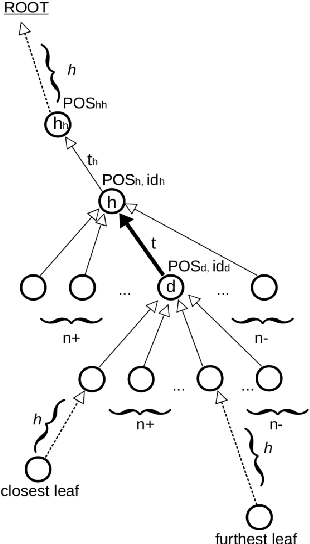
\includegraphics[scale=0.5]{img/lisca_stats.png}
    \caption[Features Used by LISCA to Calculate Plausibility Score for an Arc]{Features Used by LISCA to Calculate Plausibility Score for an Arc (marked in bold). Figure borrowed from \cite{alzetta2017dangerous}. }
\end{reusefigure}

The goal of the experiment is two-fold. For the low-resource languages, when there is no reference corpus, LISCA cannot be used directly. A common approach used in the case of low-resource languages, \(k\)-fold cross-validation is explored in this experiment. However, just using cross-validation is not enough, as the choice of the number of folds can affect the results significantly. In this experiment, we therefore (i) evaluate if \(k\)-fold cross-validation is an optimal strategy against the approach of keeping the test and train data separated, and (ii) try to map the behaviour of the algorithm to the choice of the number of folds in \(k\)-fold cross-validation approach.

In the following subsections, we shall elaborate on the experiment with LISCA. We start with the specification of the dataset to be used for the experiment in section \ref{data:lisca}, followed by the elaboration on experimental setup in section \ref{preprocess:lisca}. Section \ref{arcs:focus} specifies the manner of investigation for the analysis of arcs. We report the preliminary statistics on different runs in section \ref{baseline:lisca}, before diving into an analysis of the results in section \ref{compare:lisca}. Section \ref{typologies:lisca} deals with the typologies of errors discovered over the complete experiment. The chapter concludes with a discussion on the findings of the experiment in section \ref{results:lisca}.

\section{Dataset}
\label{data:lisca}

The experiment was conducted entirely on data from \verb|hi|-HDTB treebank from UDv2.4\footnote{Code alongwith manually annotated data is available at \url{https://github.com/Akshayanti/Masters-Thesis-CUNI-2020/tree/master/lisca_coldstart}} \citep{UDv2.4}. The motivation behind the limiting of the dataset to a particular language is threefold. Firstly, the treebank in question is limited to news genre. The lack of variability in the genre in the treebank can be used to frame a better statistical model than when there would be different genres present. Secondly, the treebank is medium sized (16,000+ sentences containing around 350k tokens) as can be seen in Table \ref{tab:hi_size2}. The medium sized treebank is optimal in the manner that a variety of values (of the number of folds in \(k\)-fold cross validation procedure) can be experimented with. Furthermore, the different values of the parameter can be used to ascertain the performance of the algorithm in both large-sized and small-sized treebanks. Lastly, the author has \verb|hi| as their native language, making it easier for them to analyse the given data, thus reducing the source of ambiguity during the process of manual annotation and verification of results from the results of the algorithm.

\begin{table}[H]
    \centering
    \begin{tabular}{|c|c|c|}
    \hline
    \textbf{Split} & \textbf{Sentences} & \textbf{Tokens}\\
    \hline
    \hline
    \textbf{dev} & 1 659 & 35 217\\
    \textbf{test} & 1 684 & 35 430\\
    \textbf{train} & 13 304 & 281 057\\
    \hline
    \hline
    \textbf{Total} & \textbf{16 647} & \textbf{351 704}\\
    \hline
    \end{tabular}
    \caption{Size of \texttt{hi}-HDTB treebank}
    \label{tab:hi_size2}
\end{table}

\section{Experimental Setup}
\label{preprocess:lisca}

For the remainder of the experiment, we adapt the usage of \textit{iteration} and \textit{run} as follows. The results of one \textit{run} would be analysed together. For a given \(k\) value in \(k\)-fold cross validation, the experimental data is split into \(k\) different folds, running \(k\) \textit{iterations} for one run. 

For the different runs of the current experiment, the total number of sentences poses a problem in the terms of how many folds the data can be split into\footnote{16,647 can be factorised as 3 x 31 x 179, which allows limited manipulation in the number of folds that can be worked with for equal distribution of instances.}. To combat this problem, we first concatenate the different splits of the treebank into one. The concatenated split is then downsampled to 16,000 sentences. This downsampled data becomes our functional dataset for the experiment. The downsampling is needed to allow for the different values of \(k\) to work. While the data if downsampled to 16,640 instances would have also worked, we chose to set the count to 16,000 sentences for empirical reasons. The number of sentences from the original splits that feature in the downsampled version are as listed in Table \ref{tab:split_lisca_downsample}.

\begin{table}[H]
    \centering
    \begin{tabular}{|l||c|c||c|c|}
    \hline
    \multicolumn{1}{|c||}{\textbf{Split Name}} &
    \multicolumn{2}{c||}{\textbf{Sentences}} &
    \multicolumn{2}{c|}{\textbf{Tokens}}\\
     & \textbf{Before} & \textbf{After} & \textbf{Before} & \textbf{After}\\
    \hline
    \textbf{dev} & 1 659 & 1 601 & 35 217 & 33 964\\
    \textbf{test} & 1 684 & 1 614 & 35 430 & 33 981\\
    \textbf{train} & 13 304 & 12 785 & 281 057 & 270 249\\
    \hline
    \hline
    \textbf{Total} & 16 647 & 16 000 & 351 704 & 338 194\\  
    \hline
    \end{tabular}
    \caption{Counts of Sentences and Tokens from Individual Splits, Before and After Downsampling}
    \label{tab:split_lisca_downsample}
\end{table}

\subsubsection{Setup for Baseline Run}

We call an arc as belonging to downsampled train data if (i) the arc was part of the train set in the original data, and (ii) the arc is present in the downsampled data as well. The arcs belonging to downsampled dev data and downsampled test data are also defined similarly.

For establishing a baseline, we train the algorithm on downsampled dev and downsampled train sets, concatenated together. The trained algorithm is then run against the downsampled test data to get the plausibility score of the individual arcs present therein.

\subsubsection{Setup for Experimental Runs}

The experiments were conducted on 3 different values of \(k\). The chosen values were \(k = \{2, 4, 8\}\). When the values of \( k \geq 10\) were considered, the resulting data folds became smaller enough to not yield satisfactory results.

For each value of \(k\), the cross-validation procedure was applied to get the plausibility scores for the arcs in the entire downsampled dataset. The LISCA algorithm for each iteration was run by \citeauthor{alzetta2017dangerous} separately. Algorithm \ref{algo:liscadata} summarises the procedure involved so far.

\begin{algorithm}[H]
\caption{Experimental Setup for \(k\)-fold Cross Validation}
\label{algo:liscadata}
    \begin{algorithmic}[1]
    \REQUIRE Downsampled \texttt{hi}-HDTB Treebank $T$
    \FORALL{$k$ in \{2, 4, 8\}}
        \STATE $T.folds \leftarrow \{T.1$, ..., $T.k\}$ subject to conditions:
        \STATE $T = \bigcup \{T.1, ..., T.k\}$ \COMMENT{Condition 1}
        \STATE $sentences(T.i) = sentences(T)/k \hspace{2mm} \forall T.i \in T$
        \COMMENT{Condition 2}
        \STATE $\bigcap \{T.x1, T.x2\} = \phi \hspace{2mm} \forall \{T.x1, T.x2\}  \in T.folds$ \COMMENT{Condition 3}
        \FOR{$iteration$ in 1, ..., k}
            \STATE $fold.test \leftarrow T.iteration$
            \STATE $fold.training \leftarrow T - T.iteration$
            \STATE $lisca.iteration \leftarrow$ trained LISCA model on $fold.training$
            \STATE $lisca.iteration$ is used to assign plausibility score to arcs in $fold.test$
        \ENDFOR
    \ENDFOR
    \end{algorithmic}
\end{algorithm}

\section{Arcs in Focus}
\label{arcs:focus}

The evaluation of a trained LISCA model on a given test data generates several types of statistics. In addition, the individual arcs in the results of the LISCA algorithm are split into 10 equal bins in descending order of their plausibility scores, with an additional bin for the remnants. The statistics are presented on a per-bin basis and include POS distribution, deprel distribution, POS and deprel distribution, syntactic link length distribution, among others. While the per-bin statistics are a useful feature, the cross validation process in the context of current experiment does not need such per-bin statistics. Instead we focus on individual arcs and their plausibility scores in the current experiment.

Henceforth, we call a particular arc as flagged in a particular run if its plausibility score in the run is designated as 0, i.e. the arc is deemed as improbable by the run. While \cite{alzetta2017dangerous} looked at all the instances in the last two bins (and the extra remnant bin), the current setup narrows down the search scope. The last two (and the extra remnant) bins in question are the only ones containing arcs with 0-score or with scores that are very close to 0. As we would show later (in section \ref{statistics:experiments}), the scores for non-zero scored arcs would fluctuate with different datasets of the same language, or even based on the number of folds in cross validation. This can be extrapolated to state that the non-zero scored arcs in the bins in question can also vary in their scores, making the bin-specific treatment incomparable across different runs. In contrast, looking at zero-scored arcs gives us a uniform base for analysis throughout, considering that the arc was marked as improbable, and not probable with a low score.

\section{Statistics}
\label{baseline:lisca}

\subsection{Baseline Run}
\label{statistics:baseline}

The baseline run tried to find the low-probability arcs in the downsampled test data. Table \ref{tab:stats_baseline} shows the basic statistics of the run.

\begin{table}[H]
    \centering
    \begin{tabular}{|l|l|}
        \hline
        \textbf{Statistic} & \textbf{Count / Value} \\
        \hline
        Min Score & 0.00\\
        Max Score & 1.82 E-07\\
        Flagged Arcs (in \%) & 221 (0.7 \%)\\
        Total Arcs & 33 739\\
        \hline
    \end{tabular}
    \caption[Statistics for Arc Scores in Baseline Run]{Statistics for Arc Scores in Baseline Run. The percentage score of Flagged Arcs is calculated against the Total Arcs count.}
    \label{tab:stats_baseline}
\end{table}

Once the plausibility scores are assigned for the arcs, the flagged arcs were manually checked to see if they are erroneous or not. Of the 221 flagged arcs in the run, 110 arcs were found to be erroneous. The complete typology of the errors is reserved for later. However, Table \ref{tab:base_error_breakdown} shows the classification of errors from the run into Random or Systemic Errors.

\begin{table}[H]
    \centering
    \begin{tabular}{|l|c|}
        \hline
        \textbf{Statistic} & \textbf{Count (\% Total Arcs)}\\
        \hline
        No Error & 111 (49.3 \%)\\
        Systemic Errors & 96 (43.4 \%)\\
        Random Errors & 14 (6.3 \%)\\
        Total Flagged Arcs & 221\\
        \hline
    \end{tabular}
    \caption{Classification of Errors in Baseline Run}
    \label{tab:base_error_breakdown}
\end{table}


\subsection{Experimental Runs}
\label{statistics:experiments}

Table \ref{tab:absminmax} shows the number of arcs that were flagged across different experimental runs. As mentioned earlier, the maximum plausibility score of arcs in a given run fluctuates with the different \(k\)-values across different runs, even when the overall experimental data remains the same.

\begin{table}[H]
    \centering
    \begin{tabular}{|c|c|c|c|c|}
    \hline
    \textbf{\(k\)-value} & \textbf{Min Score} & \textbf{Max Score} & \textbf{0-score arcs} & \textbf{Total arcs}\\
    \hline
    \hline
    2 & 0.00 & 1.96 E-07 & 3 487 & 336 079 \\
    4 & 0.00 & 1.93 E-07 & 2 620 & 336 079 \\
    8 & 0.00 & 1.91 E-07 & 2 319 & 336 079 \\
    \hline
    \end{tabular}
    \caption{Statistics for Arc Scores in Experimental Runs}
    \label{tab:absminmax}
\end{table}

The number of 0-scored arcs went down with an increasing \(k\)-value. In addition, all the arcs flagged in a particular run were also present in a run with a lower \(k\)-value, i.e. the arcs flagged in run with \(k=4\) were also present in \(k=2\). Similarly, the arcs flagged in run with \(k=8\) were present in the run with \(k=4\) as well as one with \(k=2\). We compare the performance of the different experimental runs against each other in section \ref{analysis:all}.

\section{Analysis}
\label{compare:lisca}

In this section, we analyse the experiment in two parts. In the first part of the analysis (Section \ref{analysis:test}), we check the usefulness of \(k\)-fold cross validation against the arcs from only the downsampled test data, comparing them at the same time. The primary motive of this analysis is to understand how the cross validation technique performs in relation to the baseline approach at identifying erroneous instances in a low-resource setting.

In the second part of the analysis (Section \ref{analysis:all}), we look at all the arcs that are flagged in different cross validation runs, regardless of them belonging to the downsampled test, dev or train data. The motive of this analysis is to understand how the difference in number of folds during cross validation affects the flagged instances.

\subsection{Baseline vs Cross Validation: Who did it better?}
\label{analysis:test}

Table \ref{tab:test_lisca} shows the number of test arcs that were flagged across different cross validation runs. The values in the last column represent the count of instances that were flagged by the experimental run as well as the baseline run. 

\begin{table}[H]
    \centering
    \begin{tabular}{|c||c|c|c|c|}
    \hline
    \multicolumn{1}{|c||}{\textbf{\(k\)-value}} &
    \multicolumn{1}{c|}{\textbf{\# Flagged}} &
    \multicolumn{1}{c|}{\textbf{\# Also Flagged by Baseline}}\\
     & & \textbf{(\% \# Flagged)}\\
    \hline
    2 & 333 & 211 (63.36\%) \\
    4 & 254 & 205 (80.71\%) \\
    8 & 226 & 205 (90.71\%) \\
    \hline
    \end{tabular}
    \caption{Commonly Flagged Instances from Downsampled Test Data in Baseline and Experimental Runs}
    \label{tab:test_lisca}
\end{table}

Table \ref{tab:baseline_cv_error_percentage} shows the counts of arcs in downsampled test data that were flagged across different runs, and the count of flagged arcs that were erroneous.

\begin{table}[H]
    \centering
    \begin{tabular}{|c|c|c|c|}
    \hline
    \textbf{Run} & \textbf{\# Flagged} & \textbf{\# Errors} & \textbf{Error Precision (in \%)}\\
    \textbf{ } & \textbf{(TP+FP)} & \textbf{TP} & \textbf{TP*100/(TP+FP)}\\
    \hline
    Baseline & 221 & 109 & 49.32 \%\\
    Experimental (\(k=2\)) & 333 & 160 & 48.05 \%\\
    Experimental (\(k=4\)) & 254 & 127 & 50.00 \%\\
    Experimental (\(k=8\)) & 226 & 114 & 50.44 \%\\
    \hline
    \end{tabular}
    \caption{Error Counts in Downsampled Test Data across Different Runs}
    \label{tab:baseline_cv_error_percentage}
\end{table}

Table \ref{tab:baseline_cv_error_percentage} can be analysed in two different ways. The first analysis would focus on the error precision for each run. We notice that an increase in \(k\)-value in cross-validation approach results in an increasing precision. While the experimental run with \(k=2\) had a precision lower than the precision of the baseline run (\(\Delta = -1.27 \%\)), the other experimental runs had a higher precision than the baseline run (\(\Delta = 0.68 \%\) for \(k=4\) and \(\Delta = 1.12 \%\) for \(k=8\)). In this aspect, cross-validation technique still outperforms the trivial technique used in the baseline task. However, the choice of \(k\)-value in this case needs to be monitored for a higher precision.

The second analysis of data in Table \ref{tab:baseline_cv_error_percentage} would essentially focus on the number of identified erroneous arcs in the individual run. Considering that we are interested in a higher number of error arcs, either of the experimental runs outperform the baseline task in that aspect as well.

We therefore are able to establish that the cross-validation technique is a better choice than the trivial approach. Table \ref{tab:typology_test_arcs} shows the typology of different errors as identified in the different runs. We discuss the most relevant error typologies in Section \ref{typologies:lisca}.

\begin{table}[H]
    \scalebox{0.95}{\begin{tabular}{|l|c|c|c|c|}
    \hline
    \textbf{Error Typology} & \textbf{Baseline} & \textbf{\(k=2\)} & \textbf{\(k=4\)} & \textbf{\(k=8\)}\\
    \hline
        \texttt{advcl4advmod} & 2 (0.9\%) & 2 (0.6\%) & 2 (0.8\%) & 2 (0.9\%)\\
        \texttt{advcl4det} & - & 2 (0.6\%) & - & -\\
        \texttt{amod4acl} & 2 (0.9\%) & 3 (0.9\%) & 2 (0.8\%) & 2 (0.8\%)\\
        \textbf{\texttt{amod4xcomp}} & 2 (0.9\%) & 3 (0.9\%) & 3 (1.2\%) & 2 (0.9\%)\\
        \texttt{compound4det} & - & 2 (0.6\%) & 1 (0.4\%) & 1 (0.4\%)\\
        \texttt{compound4obj} & 1 (0.5\%) & 2 (0.6\%) & 2 (0.8\%) & 2 (0.9\%)\\
        \textbf{\texttt{nmod4obl}} & - & 4 (1.2\%) & 2 (0.8\%) & 1 (0.4\%)\\
        \textbf{\texttt{obl4advcl|acl}} & 1 (0.5\%) & 2 (0.6\%) & 2 (0.8\%) & 1 (0.4\%)\\
        \texttt{obl4discourse|mark} & - & 3 (0.9\%) & 1 (0.4\%) & -\\
        \texttt{Case Error} & 5 (2.3\%) & 6 (1.8\%) & 5 (2.0\%) & 5 (2.2\%)\\
        \texttt{MWE Error} & 5 (2.3\%) & 5 (1.5\%) & 5 (2.0\%) & 5 (2.2\%)\\
        \texttt{Naming Error} & 9 (4.1\%) & 11 (3.3\%) & 9 (3.5\%) & 8 (3.5\%)\\
        \texttt{POS Error} & 5 (2.3\%) & 5 (1.5\%) & 3 (1.2\%) & 3 (1.3\%)\\
        \texttt{Reported Speech} & 4 (1.8\%) & 2 (0.6\%) & 2 (0.8\%) & 2 (0.9\%)\\
        \texttt{Tree Error} & 20 (9.0\%) & 29 (8.7\%) & 25 (9.8\%) & 22 (9.7\%)\\
        \texttt{Wrong Head} & 38 (17.2\%) & 54 (16.2\%) & 42 (16.5\%) & 40 (17.7\%)\\
        Random Errors & 15 (6.8\%) & 25 (7.5\%) & 21 (8.3\%) & 18 (8.0\%)\\
        No Error & 112 (50.7\%) & 173 (50.0\%) & 127 (50.0\%) & 112 (49.6\%)\\
    \hline
        \textbf{Total Flagged Arcs} & \textbf{221} & \textbf{333} & \textbf{254} & \textbf{226}\\
    \hline
    \end{tabular}}
    \caption[Typology of Errors in Downsampled Test Data across Different Runs]{Typology of Errors in Downsampled Test Data across Different Runs. Percentages are calculated against the Total number of Flagged Arcs in the Run. Error Typologies marked in bold have been previously pointed out by \cite{alzetta2017dangerous}}
    \label{tab:typology_test_arcs}
\end{table}

\subsection{Comparing Different Experimental Runs}
\label{analysis:all}

For the analysis of the different cross-validation runs, we noticed that the count of flagged instances decreased with the increase in the number of folds. We hypothesise that as we increase the number of folds, the detection of rare errors improves while the detection of frequent errors deteriorates. having noted this, we analysed the effect of each k-value in the following manner. For the 0-scored arcs that were common to all the runs, 200 randomly chosen arcs (out of 2319) were evaluated manually. Out of the arcs common only to the runs corresponding to \(k= \{2, 4\}\), 100 were randomly chosen for manual evaluation. Finally, 100 of the arcs that are local only to the run corresponding to \(k=2\) were chosen randomly for manual evaluation. The manual evaluation on a flagged instance was meant to classify if the flagged instance is indeed an error, and if so, of what kind.

The manual annotation on limited subsamples as above does not offer a comparative viewpoint of the performance of the different runs. To combat this, we estimate the normalized frequency of each error type over 1000 instances in Table \ref{tab:normalized_experimental_lisca}. The values are calculated as per the equation given below. The equation normalizes the frequency of an error over 1000 flagged arcs, based on the distribution of the error in the annotated samples.

    \[f_{error} = 
    \begin{cases}
    k_{2,4,8} \cdot 5 &\text{for }k=8\\
    \vspace{2mm}\\
    \left[ \frac{k_{2,4,8} \cdot 2319}{200} + \frac{k_{2,4} \cdot 311}{100} \right] \cdot \frac{1000}{2620} & \text{for }k=4\\
    \vspace{2mm}\\
    \left[ \frac{k_{2,4,8} \cdot 2319}{200} + \frac{k_{2,4} \cdot 311}{100} + \frac{k_{2} \cdot 867}{100} \right] \cdot \frac{1000}{3487} & \text{for }k=2
    \end{cases}\]
where
\begin{itemize}
    \item \(f_{error}\) represents the normalised frequency of \(error\)
    \item \(k_{2,4,8}\) represents the counts of \(error\) in the annotated sample of arcs commonly flagged by all the experimental runs
    \item \(k_{2,4}\) represents the counts of \(error\) in the annotated sample of arcs commonly flagged by runs with \(k=2\) or \(k=4\), but not flagged by run with \(k=8\)
    \item \(k_{2}\) represents the counts of \(error\) in the annotated sample of arcs flagged only by the run with \(k=2\), but not flagged by runs with \(k=4\) or \(k=8\)
\end{itemize}

\begin{table}[H]
    \centering
    \begin{tabular}{|l|c|c|c|}
        \hline
        \textbf{Error Typology} & \textbf{\(k = 2\)} & \textbf{\(k= 4\)} & \textbf{\(k=8\)} \\
        \hline
        \texttt{advmod4amod} & 7 & 9 & 10\\
        \texttt{dep4det} & 6 & 8 & 5\\
        \texttt{dep4discourse|mark} & 6 & 5 & 5\\
        \texttt{nsubj4obj} & 8 & 7 & 5\\
        \textbf{\texttt{obl4advcl|acl}} & 6 & 8 & 5\\
        \texttt{Case Error} & 16 & 8 & 5\\
        \texttt{MWE Error} & 15 & 13 & 15\\
        \texttt{Naming Error} & 43 & 51 & 50\\
        \texttt{POS Error} & 10 & 13 & 15\\
        \texttt{Reported Speech} & 12 & 13 & 15\\
        \texttt{Tree Error} & 47 & 61 & 60\\
        \texttt{Wrong Head} & 163 & 167 & 180\\
        Random Errors & 142 & 115 & 115\\
        No Error & 519 & 522 & 515\\
        \hline
        \textbf{Total Errors} & \textbf{481} & \textbf{478} & \textbf{485}\\
\hline
    \end{tabular}
    \caption[Error Frequencies for Experimental Runs, Normalized Over 1000 Flagged Arcs]{Error Frequencies for Experimental Runs, Normalized Over 1000 Flagged Arcs. Error Typologies marked in bold have been previously pointed out by \cite{alzetta2017dangerous}}
    \label{tab:normalized_experimental_lisca}
\end{table}

Perhaps the most striking result from Table \ref{tab:normalized_experimental_lisca} is how the different experimental runs are almost similar in their performance. Notice that in Table \ref{tab:baseline_cv_error_percentage}, an increase in number of folds was accompanied by an increase in the calculated error precision. The analysis in the two cases is different. While in Table \ref{tab:baseline_cv_error_percentage} we checked if using the cross-validation to train the algorithm has any significant performance gain; the results in Table \ref{tab:normalized_experimental_lisca} analyzes if the number of folds has any correlation with error-detection rate when there is no reference corpus, and the algorithm is trained and tested on the same data. 

Since the number of folds in cases when the algorithm is trained and tested using cross-validation has little to no effect in performance gain, the only point of differentiation between different runs is with respect to the number of flagged arcs. While it is lucrative to use less number of folds (or a lower \(k\) value), the approach would be bottle-necked by the size of the dataset.

An error type is considered significant if its normalized frequency is more than 1\% (frequency \(> 10\)) in  Table \ref{tab:normalized_experimental_lisca}. We discuss the significant error types in the next section.

\section{Error Typologies}
\label{typologies:lisca}

In this section, we elaborate on the error typologies discovered throughout the scope of the experiment such that the discovered error type is present in more than 1\% of the arcs flagged in any run, baseline or experimental. The focused errors in this section include: \texttt{Case Error}, \texttt{MWE Error}, \texttt{Naming Error}, \texttt{Reported Speech}, \texttt{Tree Error} and \texttt{Wrong Head}. Since `Random Errors' are not systemic in nature, we do not elaborate on them. Additionally, \texttt{POS Error} corresponds to an error in the POS annotation label, and is not elaborated upon any further in this section.

\subsection[Identification Error of Case-Marker: \texttt{Case Error}]{\texttt{Case Error}: Identification Error of Case-Marker}

In \texttt{hi}, the different grammatical cases are more often than not marked by case-marker tokens. This error corresponds to such case-markers being marked by deprels other than \texttt{case}. Additionally, the deprel is the preferred choice for constructions that involve possessions as well. In the event that the used deprel is other than \texttt{case}, we call it as \texttt{Case Error}.

Part of sentence from UDv2.4 \texttt{hi}-HDTB treebank in Example \ref{examp:caseError}, and the associated dependency tree in Figure \ref{examp:caseError-fig} highlights the error type. The token of interest is marked in bold.

\begin{example}
\label{examp:caseError}
\textbf{ }\\
\textbf{Text (\texttt{hi}):} \texthindi{मार्क्र्सवादी कम्युनिस्ट पार्टी ( माकपा ) \textbf{के} दस सांसदों}\\
\textbf{Translit:} \textit{Marx-vaadi Communist Party ( MaCPa ) \textbf{ke} das saansadon}\\
\textbf{Lit.:} Marxist Communist Party (MaCPa) \textit{Poss.} ten senator-\textit{Acc.}-\textit{Pl.}\\
\textbf{Translated:} 10 senators of Marxist Communist Party (MaCPa)
\end{example}

\begin{figure}[H]
    \centering
    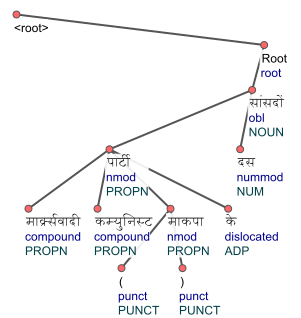
\includegraphics[scale=0.90]{img/caseError.png}
    \caption{\texttt{Case Error} in Example \ref{examp:caseError}}
    Note: Root is used as a placeholder for root of the tree\\
    Note: \texthindi{मार्क्र्सवादी} (\textit{Marx-vaadi}; Marxist) should be attached to \texthindi{पार्टी} (\textit{Party}; Party) using deprel \texttt{flat}, and not with \texttt{compound}\\
    Note: \texthindi{कम्युनिस्ट} (\textit{Communist}; Communist) should be attached to 
    \texthindi{पार्टी} (\textit{Party}; Party) using deprel \texttt{flat}, and not with \texttt{compound}\\
    Note: \texthindi{माकपा} (\textit{MaCPa}; abbreviation of Marxist Communist Party) should be attached to 
    \texthindi{पार्टी} (\textit{Party}; Party) using deprel \texttt{appos}, and not with \texttt{nmod}\\
    Note: \texthindi{के} (\textit{ke}; \textit{Poss.}) should be attached to 
    \texthindi{पार्टी} (\textit{Party}; Party) using deprel \texttt{case}, and not with \texttt{dislocated}
    
    \label{examp:caseError-fig}
\end{figure}
% test-s957

\subsection[Annotation Error in Multi-Word Expression (MWE): \texttt{MWE Error}]{\texttt{MWE Error}: Annotation Error in Multi-Word Expression (MWE)}

The different tokens in a Multi-Word Expression (MWE) are combined by either of the deprels in UDv2: \texttt{fixed}, \texttt{compound} or \texttt{flat}. Of these, \texttt{fixed} is used for completely fixed grammaticized (function word-like) MWEs (like `in spite of'), and \texttt{compound} applies to endocentric (headed) MWEs (like `apple pie').

The usage of \texttt{fixed} deprel is covered separately in \texttt{Naming Error}. For instances when a MWE should be annotated as either of \texttt{compound} or \texttt{fixed} deprels, but is annotated otherwise, we refer to the error as \texttt{MWE Error}. Example \ref{examp:mweError} shows the error type in a sentence from UDv2.4 \texttt{hi}-HDTB treebank, with the associated dependency tree in Figure \ref{examp:mweError-fig}. The MWE is marked in bold.

\newpage
\begin{example}
\label{examp:mweError}
\textbf{ }\\
\textbf{Text (\texttt{hi}):} \texthindi{इसकी सबसे बड़ी विशेषता यह है कि सामान्य कार्य चलता रहेगा और किसी चीज की प्रोसेसिंग भी \textbf{अपने आप} होती रहेगी ।}\\
\textbf{Translit:} \textit{iski sabse badi visheshta yeh hai ki saamaanya kaarya chaltaa rahegaa aur kisi cheej ki processing bhi \textbf{apne aap} hoti rahegi.}\\
\textbf{Lit.:} \textcolor{red}{\textit{3P.Poss.} \textit{Superlative} big feature this is that normal work run-\textit{Imp.} \textit{Fin.} and some thing \textit{Poss.} process also by-itself}\\
\textbf{Translated:} \textcolor{red}{Need to ask for translation}
\end{example}

\begin{figure}[H]
    \centering
    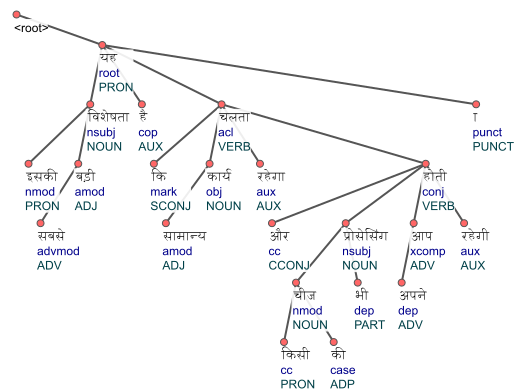
\includegraphics[scale=0.90]{img/mweError.png}
    \caption{\texttt{MWE Error} in Example \ref{examp:mweError}}
    Note: \texthindi{अपने} (\textit{apne}; ?) should be connected to \texthindi{आप} (\textit{aap}; ?) using deprel \texttt{fixed}, and not \texttt{dep}
    \label{examp:mweError-fig}
\end{figure}
% train-s1411

\subsection[Annotation Error in Construction With Reported Speech: \texttt{Reported Speech}]{\texttt{Reported Speech}: Annotation Error in Construction With Reported Speech}

According to UDv2 guidelines for treatment of reported speech\footnote{\url{https://universaldependencies.org/u/dep/parataxis.html\#treatment-of-reported-speech}}, the reported speech is connected to the main clause by using either of the deprel \texttt{ccomp} or \texttt{parataxis}.

The error \texttt{Reported Speech} corresponds to case when the reported speech and main clause are not connected by proper deprels, as in the example from UDv2.4 \texttt{hi}-HDTB treebank.

\begin{example}
\label{examp:reportedSpeech}
\textbf{ }\\
\textbf{Text (\texttt{hi}):} \texthindi{समिति ने कहा था कि सभी संस्थान मौजूदा आईआईटी के स्तर की तुलना में काफी पीछे हैं ।}\\
\textbf{Translit:} \textit{samiti ne kahaa thaa ki sabhi sansthaan maujoodaa IIT ke star ki tulnaa mei kaafi peeche hain.}\\
\textbf{Lit.:} Committee \textit{Acc.} say be-\textit{Perf.} that all institutes present IIT \textit{Poss.} level in-comparison-with quite behind is-\textit{Pl.} . \\
\textbf{Translated:} Committee had said that all institutes are far behind the level of the current IITs. 
\end{example}

\begin{figure}[H]
    \centering
    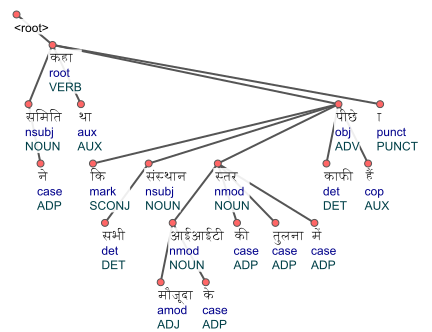
\includegraphics[scale=0.90]{img/reportedSpeech.png}
    \caption{\texttt{Reported Speech Error} in Example \ref{examp:reportedSpeech}}
    Note: \texthindi{पीछे} (\textit{peeche}; behind) should be attached to 
   \texthindi{कहा} (\textit{kaha}; say) using the deprel \texttt{ccomp}
    \label{examp:reportedSpeech-fig}
\end{figure}
% test-s1055

\subsection[Head Identification Error: \texttt{Wrong Head}]{\texttt{Wrong Head}: Head Identification Error}

The error refers to the cases when the dependent in the flagged arc is attached to a wrong head. This is the umbrella error type for all the cases of head identification error that cannot be categorised more specifically into other error types.

While \cite{alzetta2017dangerous} mention head labelling error as a sub-type of the error patterns discussed therein, we identify this error in a category on its own. We separate this error type because multiple parsers/taggers determine the deprel of a dependent in an arc based on the head of the said dependent. Keeping this in mind, \texttt{Wrong Head} is very likely to result in a faulty deprel annotation as well. However, attachment to the correct head in this case should essentially result in a correction of the annotated deprel as well.

Consider Example \ref{examp:wrongHead} and the associated dependency tree in Figure \ref{examp:wrongHead-fig}. The example is part of a sentence taken from the UDv2.4 \texttt{hi}-HDTB treebank, and shows the token of interest (marked in bold) attached to a wrong head.

\begin{example}
\label{examp:wrongHead}
\textbf{ }\\
\textbf{Text (\texttt{hi}):} \texthindi{जिनकी \textbf{मदद} से \textbf{वह आवाज} को पहचान व समझ सकता है}\\
\textbf{Translit:} \textit{jinki \textbf{madad} se \textbf{vah aavaaz} ko pehchaan va samajh saktaa hai}\\
\textbf{Lit.:} whose help \textit{Acc.} it sound \textit{Acc.} recognise and understand can is\\
\textbf{Translated:} With help of which, it can recognise and understand sound.
\end{example}

\begin{figure}[H]
    \centering
    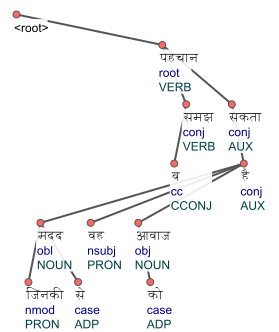
\includegraphics[scale=0.90]{img/wrongHead.png}
    \caption{Head Identification Error in Example \ref{examp:wrongHead}}
    Note: \texthindi{मदद} (\textit{madad}; help) should be attached to \texthindi{पहचान} (\textit{pehchaan}; recognise) and not to \texthindi{है} (\textit{hai}; is)\\
    Note: \texthindi{वह} (\textit{vah}; it) should be attached to \texthindi{पहचान} (\textit{pehchaan}; recognise) and not to \texthindi{है} (\textit{hai}; is)\\
    Note: \texthindi{आवाज} (\textit{aavaz}; sound) should be attached to \texthindi{पहचान} (\textit{pehchaan}; recognise) and not to \texthindi{है} (\textit{hai}; is)\\
    \label{examp:wrongHead-fig}
\end{figure}
% test-s1083

\subsection[Annotation Error in Proper Nouns: \texttt{Naming Error}]{\texttt{Naming Error}: Annotation Error in Proper Nouns}

\texttt{Naming Error} is often accompanied with a head-identification error. Annotation Errors in Proper Nouns can be of three kinds, and all of these are commonly grouped under \texttt{Naming Error}. The following are the possible cases of error in annotation:

\begin{enumerate}

    \item \textbf{Proper Noun as Appositional Modifier} (\texttt{4appos}): The deprel \texttt{appos}\footnote{\url{https://universaldependencies.org/u/dep/appos.html}} is used when the proper noun defines, modifies, names or describes a preceding nominal. It also includes parenthesized examples, and the abbreviations. This error is characterized by an attempt to connect the two nominals by relations such as \texttt{nmod}, when the actual deprel should be \texttt{appos}.
    
    \item \textbf{Names/Dates without Syntactic Structure} (\texttt{4flat}): The different parts of a single name, or of a date should be attached to the head with the deprel \texttt{flat}\footnote{\url{https://universaldependencies.org/u/dep/flat.html}}. The deprel is also used in cases of a honorofic or a title. This error type is characterized by usage of other deprels when \texttt{flat} should be the deprel of choice.

    \item \textbf{Names with Syntactic Structure}: Names that follow a syntactic structure (like `A Tale of Two Cities') should not be annotated with \texttt{flat} deprel, but with regular syntactic relations. In this case, the error is characterized by a name with syntactic structure being analysed in the same way as a name without syntactic structure.
    
\end{enumerate}

Consider the part of a sentence from UDv2.4 \texttt{hi}-HDTB treebank showcasing all the above cases in Example \ref{examp:namingError} and the associated dependency tree in Figure \ref{examp:namingError-fig}
\begin{example}
\label{examp:namingError}
\textbf{ }\\
\textbf{Text (\texttt{hi}):} \texthindi{आरसी मिश्रा की पुस्तक 'मानवाधिकार संरक्षण विशेष संदर्भ, अपराधियों का निरोध एवं उपचार'}\\
\textbf{Translit:} \textit{Aarsi Mishra ki pustak ` Maanavadhikar sanrakshan vishesh sandarbh , apraadhiyon ka nirodh evam upchaar '}\\
\textbf{Lit.:} Aarsi Mishra \textit{Poss.} book ` Human-Rights Protection Special Reference , criminal-\textit{Pl.} \textit{Acc.} prevention and cure '\\
\textbf{Translated:} Aarsi Mishra's book, `Maanavadhikar sanrakshan vishesh sandarbh , apraadhiyon ka nirodh evam upchaar'
\end{example}

\begin{figure}[H]
    \centering
    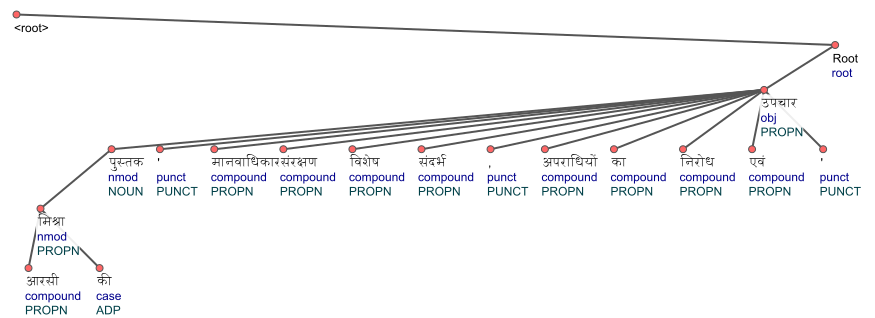
\includegraphics[scale=0.60]{img/namingError.png}
    \caption{\texttt{Naming Error} in Example \ref{examp:namingError}}
    Note: Root is used as a placeholder for root of the tree\\
    Note: \texthindi{आरसी} (\textit{Aarsi}; Aarsi) should be attached to \texthindi{मिश्रा} (\textit{Mishra}; Mishra) using deprel \texttt{flat}, and not with \texttt{compound}\\
    Note: The title of the book (limited by quotes) should be attached to \texthindi{पुस्तक} (\textit{pustak}; book) with the deprel \texttt{appos}\\
    Note: The title of the book (limited by quotes) should be annotated with regular syntactic relations
    \label{examp:namingError-fig}
\end{figure}
% test-s1183

\subsection[Dependency Head Located in Subtree: \texttt{Tree Error}]{\texttt{Tree Error}: Dependency Head Located in Subtree}

A special case of \texttt{Wrong Head} error, this error type is used for the cases when the actual head of a dependency is located inside the subtree rooted at the dependent. In order to correct the dependency, it should be essentially inverted. Essentially speaking, a tree marked with this error type requires re-annotation before any analysis can be performed on it.

Example \ref{examp:treeError} shows an instance of this error in UDv2.4 \texttt{hi}-HDTB treebank, with the associated dependency tree in Figure \ref{examp:treeError-fig}. The dependent of interest is marked in bold, and the corrected instance is as shown in Figure \ref{examp:treeError-fig2}.
\begin{example}
\label{examp:treeError}
\textbf{ }\\
\textbf{Text (\texttt{hi}):} \texthindi{आतंकियों द्वारा किसी विमान के \textbf{अपहरण} या आत्मघाती हमले को अंजाम देने की कोशिश किए जाने की खुफिया जानकारी}\\
\textbf{Translit:} \textit{aatankiyon dwara kisi vimaan ke \textbf{apharan} ya aatmghaati hamle ko anjaam dene ki koshish kiye jaane ki khufiya jaankaari}\\
\textbf{Lit.:} Terrorists by some plane \textit{Poss.} kidnap or self-harm attack \textit{Dat.} fruition give \textit{Dat.} attempt ? ? confidential information\\
\textbf{Translated:} The confidential information of attempt at some plane hijacking or suicide bombing by terrorists ...
\end{example}

\begin{figure}[H]
    \centering
    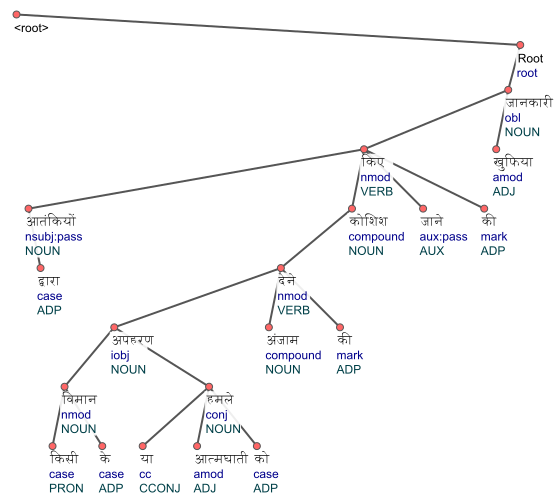
\includegraphics[scale=0.7]{img/treeError.png}
    \caption{\texttt{Subtree Error} in Example \ref{examp:treeError}}
    \label{examp:treeError-fig}
    Note: Root is used as a placeholder for root of the tree
\end{figure}

\begin{figure}[H]
    \centering
    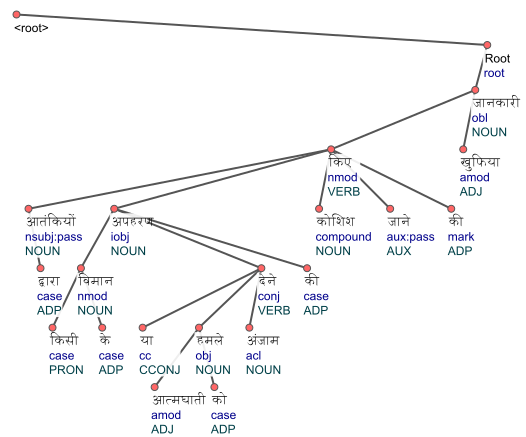
\includegraphics[scale=0.7]{img/treeError2.png}
    \caption{Correction of \texttt{Subtree Error} in Example \ref{examp:treeError}}
    \label{examp:treeError-fig2}
    Note: Root is used as a placeholder for root of the tree
\end{figure}
% dev-s1501

\section{Results and Discussion}
\label{results:lisca}

\subsection{0-scored Arcs as Search Criteria}

In their work, \cite{alzetta2017dangerous} focused on a total of 39.7k arcs in their annotation process and were finally able to manually revised 789 arcs, giving an estimated error detection rate of 2\% from the flagged instances. In our baseline run, a focus on 221 0-scored arcs led to an estimated error detection of 109 instances (49.32 \%). We must stress here that the results across the two experiments are NOT directly comparable since the treebanks used in the cited authors' experiment was of far superior quality than the one used in the current experiment. A lower quality treebank would imply a higher distribution of errors, and that could be the sole reason why the focus on a smaller subset gave a satisfactory error detection rate. Additionally, the size difference in the cited authors' work and the baseline task is another reason why the two approaches cannot be compared. We must also stress here that in our baseline approach, the search scope was lowered significantly (as compared to the experimental runs). To establish any significant difference between either approach, more experiments should be conducted with the same treebank (ensuring the quality of experimental data is a controlled variable) to establish the probability distribution of errors in 0-scored arcs and in the approach as utilised by \citeauthor{alzetta2017dangerous}.

\subsection{Cross Validation as Strategy}

Considering that the different runs perform almost similarly (Table \ref{tab:normalized_experimental_lisca}), we argue that the size of dataset used is the determining factor in selection of the number of folds in \(k\)-fold cross validation.

For less number of folds (or a lower \(k\) value), the number of flagged arcs is high, which eventually results in more errors detected. However, in case of a small dataset, the algorithm might be trained poorly if the number of folds is small. Thus, a higher number of folds (or a higher \(k\) value) is more optimal when the dataset is small in size. As the reference dataset size grows, lesser number of folds can be tried given that the algorithm can be trained well.

\subsection{Error Typologies and Annotation}

The annotations throughout the experiment were done by a single annotator. Even though inter-annotation inconsistency is a constant problem, the annotations done by a single author are even more prone to errors. While the annotations were checked multiple times, the possibility of annotation inconsistencies in manual annotation for error labelling cannot be discounted.

It is very likely for a single dependency arc to have an error that is defined separately under different labels. In such an event, the primary source of error was labelled as the error type. For example, if a dependency arc has \textit{Case Error} as well as \textit{Wrong Head} error, the former is very likely being caused by the latter. Therefore, the manual annotation for this instance would list it as a case of \textit{Wrong Head}.

Under the different head identification errors, the annotation was in the following order of priority, arranged in descending order:

\begin{enumerate}
    \item \texttt{MWE Error} or \texttt{Naming Error}
    \item \texttt{Tree Error}
    \item \texttt{Wrong Head}
\end{enumerate}

In essence, if the head identification error could not be localised to a specific error type, it was labelled under the umbrella error label of \texttt{Wrong Head}.

\subsection{Conclusion}

In the experiment, we narrowed the search scope from the bins as used by \cite{alzetta2017dangerous} to focus on the arcs that were considered as improbable by the algorithm. Additionally, we found that using cross-validation to train the algorithm has no significant performance gain.

For low-resource languages with little to no reference corpus data, we tried cross-validation approach for finding the errors. We discovered that the choice of folds in cross-validation strategy is determined by the size of the reference corpus; and in case of unavailability of one, the strategy can be used on the data itself without a significant loss in the error-detection rate. 